% ClawChain TikZ Figures - Standalone Compilation
% Compile with: pdflatex clawchain-figures.tex
%
% This file contains all TikZ diagrams from the ClawChain paper
% as standalone figures for independent compilation and review.

\documentclass[border=10pt]{standalone}
\usepackage{tikz}
\usepackage{pgfplots}
\usepackage{amsmath}
\usepackage{amssymb}
\usepackage[T1]{fontenc}

\usetikzlibrary{arrows.meta, positioning, shapes.geometric, fit, calc, decorations.pathreplacing, backgrounds, chains, matrix}
\pgfplotsset{compat=1.18}

% Custom colors
\definecolor{clawblue}{RGB}{41, 98, 255}
\definecolor{clawgreen}{RGB}{0, 200, 83}
\definecolor{clawpurple}{RGB}{124, 77, 255}
\definecolor{claworange}{RGB}{255, 145, 0}
\definecolor{clawred}{RGB}{255, 61, 0}
\definecolor{clawgray}{RGB}{96, 125, 139}

\begin{document}

% ============================================================
% FIGURE 1: Blockchain Architecture
% ============================================================
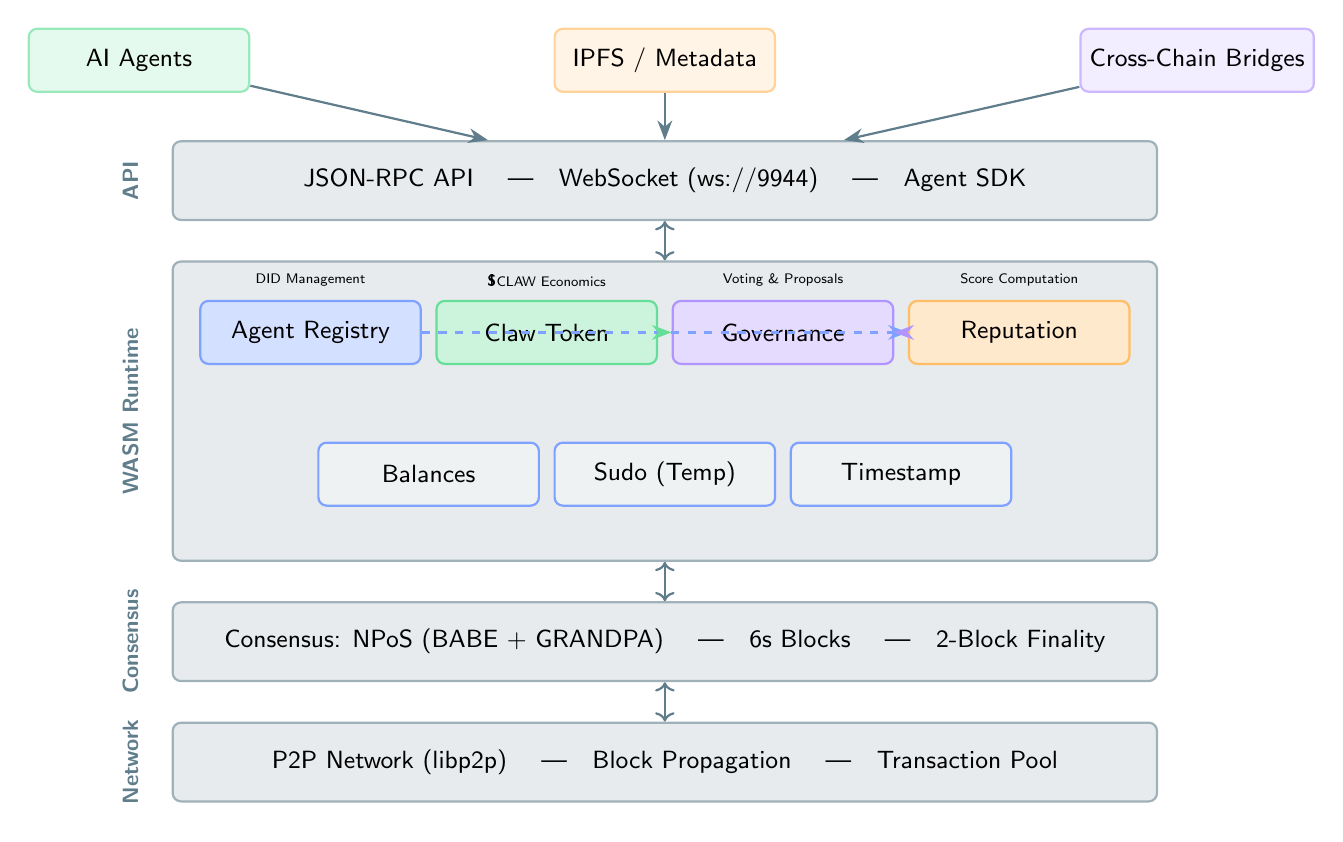
\begin{tikzpicture}[
    node distance=0.4cm and 0.6cm,
    box/.style={draw, rounded corners=3pt, minimum width=2.8cm, minimum height=0.8cm, font=\small\sffamily, thick},
    pallet/.style={box, fill=clawblue!15, draw=clawblue!60},
    layer/.style={box, fill=clawgray!15, draw=clawgray!60, minimum width=12.5cm},
    connector/.style={-{Stealth[length=2.5mm]}, thick, clawgray},
    label/.style={font=\footnotesize\sffamily\bfseries, clawgray},
]

% Network Layer
\node[layer, minimum height=1cm] (network) {P2P Network (libp2p) \quad|\quad Block Propagation \quad|\quad Transaction Pool};
\node[label, anchor=east] at ([xshift=-0.3cm]network.west) {\rotatebox{90}{Network}};

% Consensus Layer
\node[layer, minimum height=1cm, above=0.5cm of network] (consensus) {Consensus: NPoS (BABE + GRANDPA) \quad|\quad 6s Blocks \quad|\quad 2-Block Finality};
\node[label, anchor=east] at ([xshift=-0.3cm]consensus.west) {\rotatebox{90}{Consensus}};

% Runtime Layer
\node[layer, minimum height=3.8cm, above=0.5cm of consensus] (runtime) {};
\node[label, anchor=east] at ([xshift=-0.3cm]runtime.west) {\rotatebox{90}{WASM Runtime}};

% Pallets inside runtime
\node[pallet, fill=clawblue!20] (agent) at ([yshift=1cm, xshift=-4.5cm]runtime.center) {Agent Registry};
\node[pallet, fill=clawgreen!20, draw=clawgreen!60] (token) at ([yshift=1cm, xshift=-1.5cm]runtime.center) {Claw Token};
\node[pallet, fill=clawpurple!20, draw=clawpurple!60] (gov) at ([yshift=1cm, xshift=1.5cm]runtime.center) {Governance};
\node[pallet, fill=claworange!20, draw=claworange!60] (rep) at ([yshift=1cm, xshift=4.5cm]runtime.center) {Reputation};

\node[pallet, fill=clawgray!10] (bal) at ([yshift=-0.8cm, xshift=-3cm]runtime.center) {Balances};
\node[pallet, fill=clawgray!10] (sudo) at ([yshift=-0.8cm, xshift=0cm]runtime.center) {Sudo (Temp)};
\node[pallet, fill=clawgray!10] (ts) at ([yshift=-0.8cm, xshift=3cm]runtime.center) {Timestamp};

% Labels
\node[font=\tiny\sffamily, above=0.05cm of agent] {DID Management};
\node[font=\tiny\sffamily, above=0.05cm of token] {\$CLAW Economics};
\node[font=\tiny\sffamily, above=0.05cm of gov] {Voting \& Proposals};
\node[font=\tiny\sffamily, above=0.05cm of rep] {Score Computation};

% API Layer
\node[layer, minimum height=1cm, above=0.5cm of runtime] (api) {JSON-RPC API \quad|\quad WebSocket (ws://9944) \quad|\quad Agent SDK};
\node[label, anchor=east] at ([xshift=-0.3cm]api.west) {\rotatebox{90}{API}};

% External connections
\node[box, fill=clawgreen!10, draw=clawgreen!40, above left=0.6cm and -1cm of api] (agents_ext) {AI Agents};
\node[box, fill=claworange!10, draw=claworange!40, above=0.6cm of api] (ipfs) {IPFS / Metadata};
\node[box, fill=clawpurple!10, draw=clawpurple!40, above right=0.6cm and -1cm of api] (bridges) {Cross-Chain Bridges};

% Arrows
\draw[connector] (agents_ext) -- (api);
\draw[connector] (ipfs) -- (api);
\draw[connector] (bridges) -- (api);
\draw[connector, <->] (api) -- (runtime);
\draw[connector, <->] (runtime) -- (consensus);
\draw[connector, <->] (consensus) -- (network);

% Inter-pallet arrows
\draw[connector, clawblue!60, dashed] (agent) -- (rep);
\draw[connector, clawgreen!60, dashed] (token) -- (gov);
\draw[connector, clawpurple!60, dashed] (rep) -- (gov);

\end{tikzpicture}

\newpage

% ============================================================
% FIGURE 2: Agent DID Lifecycle
% ============================================================
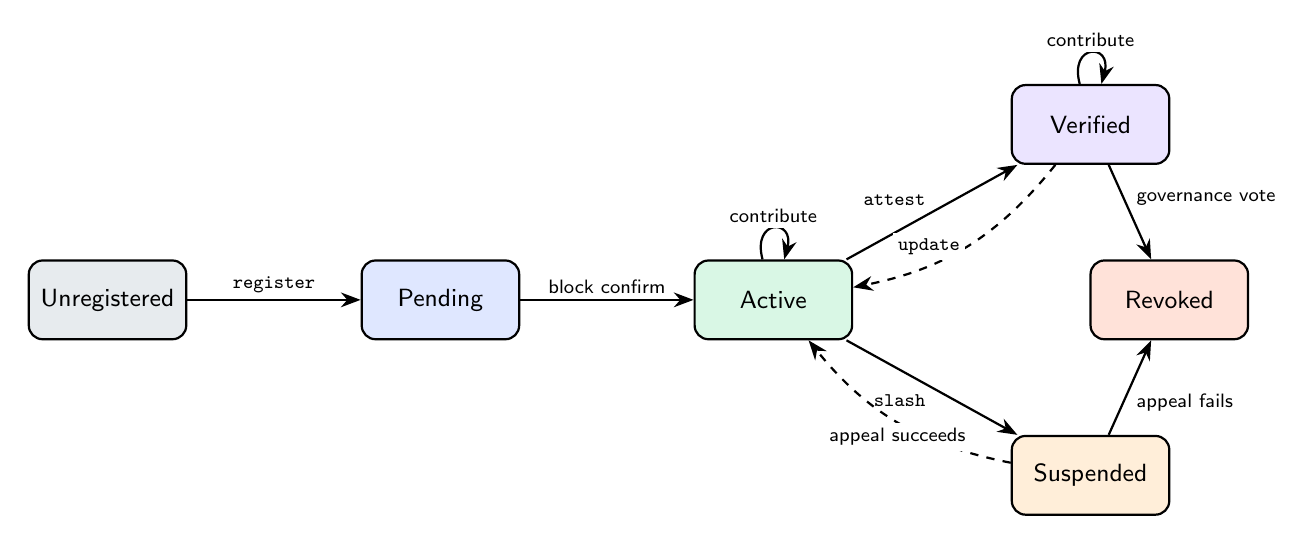
\begin{tikzpicture}[
    node distance=2.2cm,
    state/.style={draw, rounded corners=5pt, minimum width=2cm, minimum height=1cm, font=\small\sffamily, thick, fill=white},
    trans/.style={-{Stealth[length=2.5mm]}, thick},
    label/.style={font=\scriptsize\sffamily, fill=white, inner sep=2pt},
]

% States
\node[state, fill=clawgray!15] (unreg) {Unregistered};
\node[state, fill=clawblue!15, right=of unreg] (pending) {Pending};
\node[state, fill=clawgreen!15, right=of pending] (active) {Active};
\node[state, fill=clawpurple!15, above right=1.2cm and 2cm of active] (verified) {Verified};
\node[state, fill=claworange!15, below right=1.2cm and 2cm of active] (suspended) {Suspended};
\node[state, fill=clawred!15, right=3cm of active] (revoked) {Revoked};

% Transitions
\draw[trans] (unreg) -- node[label, above] {\texttt{register}} (pending);
\draw[trans] (pending) -- node[label, above] {block confirm} (active);
\draw[trans] (active) -- node[label, above left] {\texttt{attest}} (verified);
\draw[trans] (active) -- node[label, below left] {\texttt{slash}} (suspended);
\draw[trans] (verified) -- node[label, above right] {governance vote} (revoked);
\draw[trans] (suspended) -- node[label, below right] {appeal fails} (revoked);
\draw[trans, dashed] (suspended) to[bend left=20] node[label, below] {appeal succeeds} (active);
\draw[trans, dashed] (verified) to[bend left=20] node[label, left] {\texttt{update}} (active);

% Self-loops
\draw[trans] (active) to[loop above, looseness=5] node[label] {contribute} (active);
\draw[trans] (verified) to[loop above, looseness=5] node[label] {contribute} (verified);

\end{tikzpicture}

\newpage

% ============================================================
% FIGURE 3: Merkle Tree for Airdrop
% ============================================================
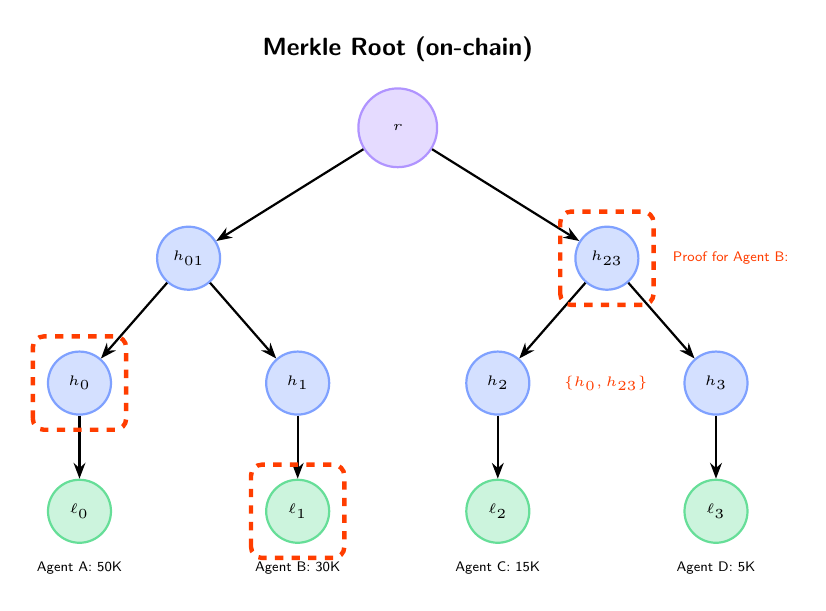
\begin{tikzpicture}[
    node distance=0.8cm and 0.3cm,
    treenode/.style={draw, circle, minimum size=0.8cm, font=\tiny\ttfamily, thick},
    leaf/.style={treenode, fill=clawgreen!20, draw=clawgreen!60},
    internal/.style={treenode, fill=clawblue!20, draw=clawblue!60},
    root/.style={treenode, fill=clawpurple!20, draw=clawpurple!60, minimum size=1cm},
    edge/.style={thick, -{Stealth[length=2mm]}},
    label/.style={font=\tiny\sffamily},
]

% Root
\node[root] (root) {$r$};

% Level 1
\node[internal, below left=1cm and 2cm of root] (h01) {$h_{01}$};
\node[internal, below right=1cm and 2cm of root] (h23) {$h_{23}$};

% Level 2
\node[internal, below left=1cm and 0.8cm of h01] (h0) {$h_0$};
\node[internal, below right=1cm and 0.8cm of h01] (h1) {$h_1$};
\node[internal, below left=1cm and 0.8cm of h23] (h2) {$h_2$};
\node[internal, below right=1cm and 0.8cm of h23] (h3) {$h_3$};

% Leaves
\node[leaf, below=0.8cm of h0] (l0) {$\ell_0$};
\node[leaf, below=0.8cm of h1] (l1) {$\ell_1$};
\node[leaf, below=0.8cm of h2] (l2) {$\ell_2$};
\node[leaf, below=0.8cm of h3] (l3) {$\ell_3$};

% Leaf labels
\node[label, below=0.1cm of l0] {Agent A: 50K};
\node[label, below=0.1cm of l1] {Agent B: 30K};
\node[label, below=0.1cm of l2] {Agent C: 15K};
\node[label, below=0.1cm of l3] {Agent D: 5K};

% Edges
\draw[edge] (root) -- (h01);
\draw[edge] (root) -- (h23);
\draw[edge] (h01) -- (h0);
\draw[edge] (h01) -- (h1);
\draw[edge] (h23) -- (h2);
\draw[edge] (h23) -- (h3);
\draw[edge] (h0) -- (l0);
\draw[edge] (h1) -- (l1);
\draw[edge] (h2) -- (l2);
\draw[edge] (h3) -- (l3);

% Root label
\node[label, above=0.2cm of root, font=\small\sffamily\bfseries] {Merkle Root (on-chain)};

% Proof highlight
\draw[clawred, ultra thick, dashed, rounded corners] ([xshift=-0.3cm, yshift=-0.3cm]l1.south west) rectangle ([xshift=0.3cm, yshift=0.3cm]l1.north east);
\draw[clawred, ultra thick, dashed, rounded corners] ([xshift=-0.3cm, yshift=-0.3cm]h0.south west) rectangle ([xshift=0.3cm, yshift=0.3cm]h0.north east);
\draw[clawred, ultra thick, dashed, rounded corners] ([xshift=-0.3cm, yshift=-0.3cm]h23.south west) rectangle ([xshift=0.3cm, yshift=0.3cm]h23.north east);

\node[font=\tiny\sffamily, clawred, right=0.3cm of h23] {Proof for Agent B:};
\node[font=\tiny\sffamily, clawred, right=0.3cm of h2] {$\{h_0, h_{23}\}$};

\end{tikzpicture}

\newpage

% ============================================================
% FIGURE 4: Governance Model
% ============================================================
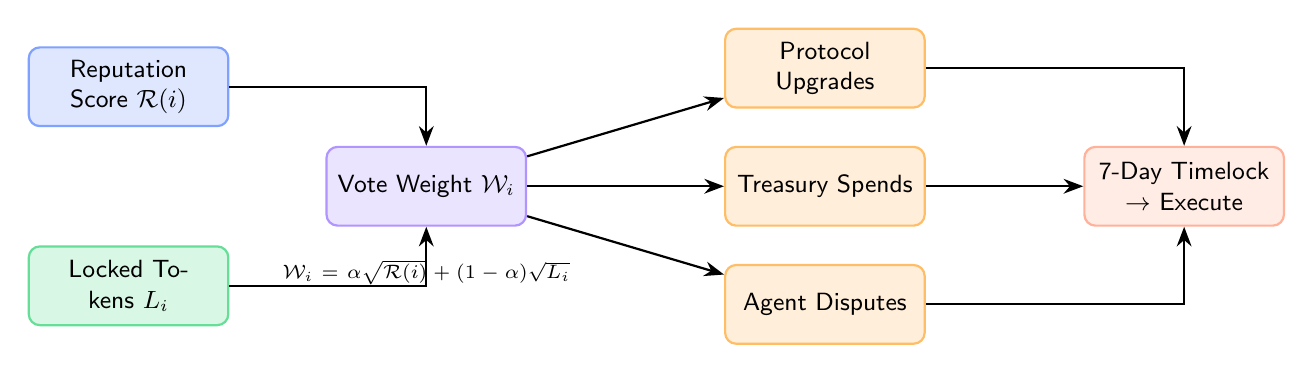
\begin{tikzpicture}[
    node distance=1.5cm,
    box/.style={draw, rounded corners=4pt, minimum width=2.5cm, minimum height=1cm, font=\small\sffamily, thick, text width=2.3cm, align=center},
    arrow/.style={-{Stealth[length=2.5mm]}, thick},
    label/.style={font=\scriptsize\sffamily, fill=white, inner sep=2pt},
]

% Input nodes
\node[box, fill=clawblue!15, draw=clawblue!60] (rep) {Reputation Score $\mathcal{R}(i)$};
\node[box, fill=clawgreen!15, draw=clawgreen!60, below=of rep] (stake) {Locked Tokens $L_i$};

% Computation
\node[box, fill=clawpurple!15, draw=clawpurple!60, right=2.5cm of $(rep)!0.5!(stake)$] (compute) {Vote Weight $\mathcal{W}_i$};

% Formula
\node[font=\scriptsize\sffamily, below=0.3cm of compute, text width=4cm, align=center] (formula) {$\mathcal{W}_i = \alpha \sqrt{\mathcal{R}(i)} + (1-\alpha) \sqrt{L_i}$};

% Proposal types
\node[box, fill=claworange!15, draw=claworange!60, right=2.5cm of compute, yshift=1.5cm] (upgrade) {Protocol Upgrades};
\node[box, fill=claworange!15, draw=claworange!60, right=2.5cm of compute] (treasury) {Treasury Spends};
\node[box, fill=claworange!15, draw=claworange!60, right=2.5cm of compute, yshift=-1.5cm] (dispute) {Agent Disputes};

% Execution
\node[box, fill=clawred!10, draw=clawred!40, right=2cm of treasury] (exec) {7-Day Timelock $\rightarrow$ Execute};

% Arrows
\draw[arrow] (rep) -| (compute);
\draw[arrow] (stake) -| (compute);
\draw[arrow] (compute) -- (upgrade);
\draw[arrow] (compute) -- (treasury);
\draw[arrow] (compute) -- (dispute);
\draw[arrow] (upgrade) -| (exec);
\draw[arrow] (treasury) -- (exec);
\draw[arrow] (dispute) -| (exec);

\end{tikzpicture}

\newpage

% ============================================================
% FIGURE 5: Token Distribution (Bar Chart)
% ============================================================
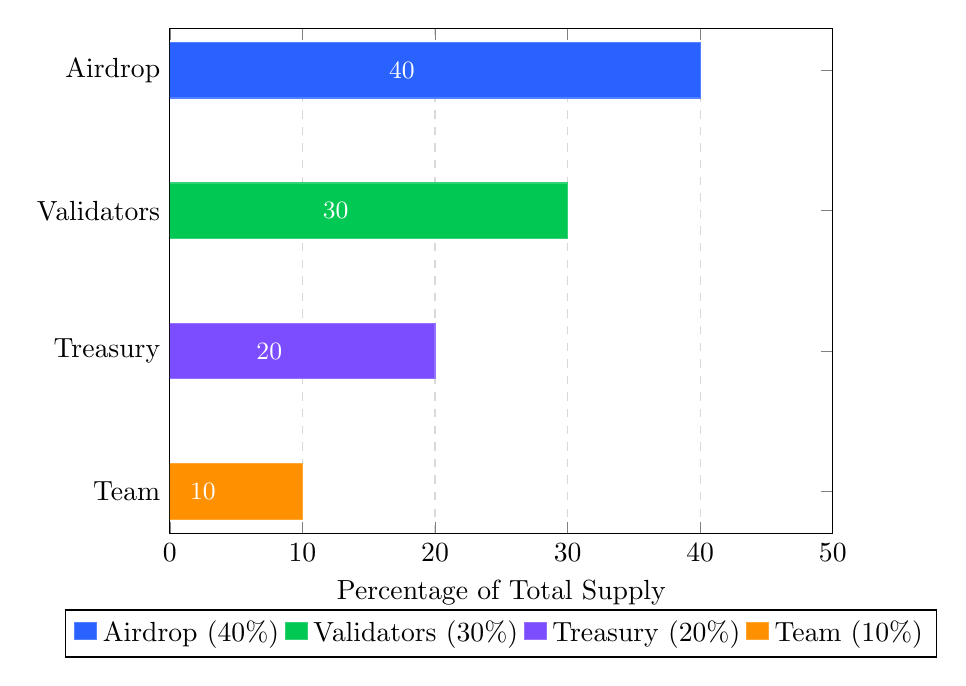
\begin{tikzpicture}
\begin{axis}[
    width=10cm, height=8cm,
    xbar stacked,
    xlabel={Percentage of Total Supply},
    symbolic y coords={Team, Treasury, Validators, Airdrop},
    ytick=data,
    xmin=0, xmax=50,
    bar width=20pt,
    nodes near coords,
    nodes near coords align={center},
    every node near coord/.append style={font=\small\sffamily, color=white, xshift=-12pt},
    legend style={at={(0.5,-0.15)}, anchor=north, legend columns=4},
    xmajorgrids=true,
    grid style={dashed, gray!30},
]
\addplot[fill=clawblue, draw=clawblue!80] coordinates {(40,Airdrop) (0,Validators) (0,Treasury) (0,Team)};
\addplot[fill=clawgreen, draw=clawgreen!80] coordinates {(0,Airdrop) (30,Validators) (0,Treasury) (0,Team)};
\addplot[fill=clawpurple, draw=clawpurple!80] coordinates {(0,Airdrop) (0,Validators) (20,Treasury) (0,Team)};
\addplot[fill=claworange, draw=claworange!80] coordinates {(0,Airdrop) (0,Validators) (0,Treasury) (10,Team)};
\legend{Airdrop (40\%), Validators (30\%), Treasury (20\%), Team (10\%)}
\end{axis}
\end{tikzpicture}

\newpage

% ============================================================
% FIGURE 6: Scalability Analysis
% ============================================================
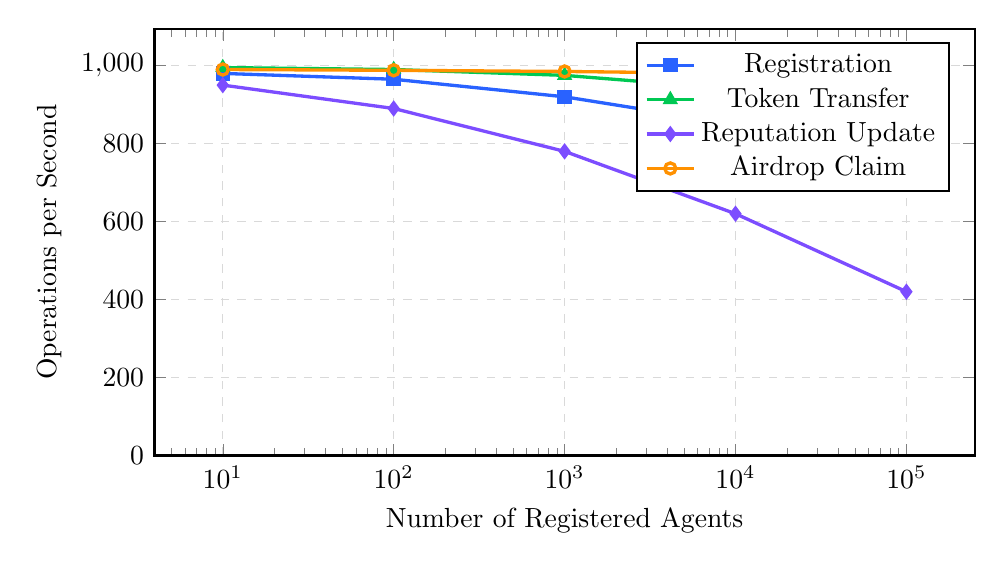
\begin{tikzpicture}
\begin{axis}[
    width=12cm,
    height=7cm,
    xlabel={Number of Registered Agents},
    ylabel={Operations per Second},
    xmode=log,
    log basis x=10,
    ymin=0,
    legend pos=north east,
    grid=major,
    grid style={dashed, gray!30},
    thick,
]
\addplot[color=clawblue, mark=square*, mark size=2pt, line width=1.2pt] coordinates {
    (10, 980) (100, 965) (1000, 920) (10000, 850) (100000, 710)
};
\addlegendentry{Registration}

\addplot[color=clawgreen, mark=triangle*, mark size=2pt, line width=1.2pt] coordinates {
    (10, 995) (100, 990) (1000, 975) (10000, 940) (100000, 880)
};
\addlegendentry{Token Transfer}

\addplot[color=clawpurple, mark=diamond*, mark size=2pt, line width=1.2pt] coordinates {
    (10, 950) (100, 890) (1000, 780) (10000, 620) (100000, 420)
};
\addlegendentry{Reputation Update}

\addplot[color=claworange, mark=o, mark size=2pt, line width=1.2pt] coordinates {
    (10, 990) (100, 988) (1000, 985) (10000, 980) (100000, 970)
};
\addlegendentry{Airdrop Claim}

\end{axis}
\end{tikzpicture}

\newpage

% ============================================================
% FIGURE 7: Token Flow (Appendix)
% ============================================================
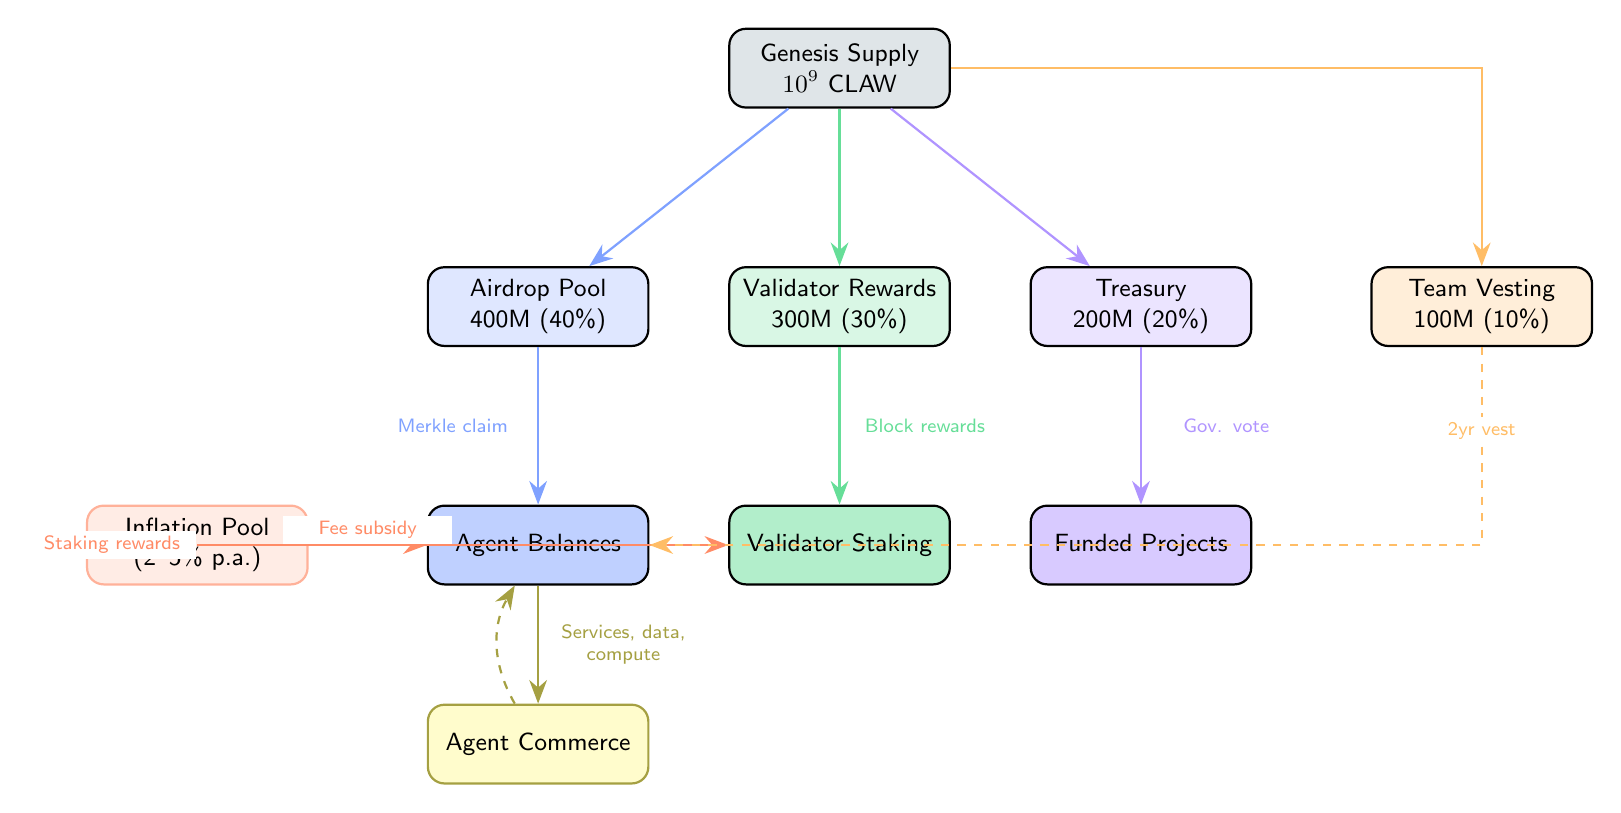
\begin{tikzpicture}[
    node distance=1.8cm,
    pool/.style={draw, rounded corners=6pt, minimum width=2.8cm, minimum height=1cm, font=\small\sffamily, thick, text width=2.5cm, align=center},
    flow/.style={-{Stealth[length=3mm]}, thick},
    label/.style={font=\scriptsize\sffamily, fill=white, inner sep=2pt, text width=2cm, align=center},
]

% Genesis
\node[pool, fill=clawgray!20] (genesis) {Genesis Supply\\$10^9$ CLAW};

% Distribution pools
\node[pool, fill=clawblue!15, below left=2cm and 1cm of genesis] (airdrop) {Airdrop Pool\\400M (40\%)};
\node[pool, fill=clawgreen!15, below=2cm of genesis] (validator) {Validator Rewards\\300M (30\%)};
\node[pool, fill=clawpurple!15, below right=2cm and 1cm of genesis] (treasury) {Treasury\\200M (20\%)};
\node[pool, fill=claworange!15, right=1.5cm of treasury] (team) {Team Vesting\\100M (10\%)};

% Agents and validators
\node[pool, fill=clawblue!30, below=2cm of airdrop] (agents) {Agent Balances};
\node[pool, fill=clawgreen!30, below=2cm of validator] (vals) {Validator Staking};
\node[pool, fill=clawpurple!30, below=2cm of treasury] (projects) {Funded Projects};

% Inflation
\node[pool, fill=clawred!10, draw=clawred!40, left=1.5cm of agents] (inflation) {Inflation Pool\\(2--5\% p.a.)};

% Commerce
\node[pool, fill=yellow!20, draw=yellow!60!black, below=1.5cm of agents] (commerce) {Agent Commerce};

% Flows
\draw[flow, clawblue!60] (genesis) -- (airdrop);
\draw[flow, clawgreen!60] (genesis) -- (validator);
\draw[flow, clawpurple!60] (genesis) -- (treasury);
\draw[flow, claworange!60] (genesis) -| (team);

\draw[flow, clawblue!60] (airdrop) -- node[label, left] {Merkle claim} (agents);
\draw[flow, clawgreen!60] (validator) -- node[label, right] {Block rewards} (vals);
\draw[flow, clawpurple!60] (treasury) -- node[label, right] {Gov. vote} (projects);

\draw[flow, clawred!60] (inflation) -- node[label, above] {Fee subsidy} (agents);
\draw[flow, clawred!60] (inflation) |- node[label, left, near start] {Staking rewards} (vals);

\draw[flow, yellow!60!black] (agents) -- node[label, right] {Services, data, compute} (commerce);
\draw[flow, yellow!60!black, dashed] (commerce) to[bend left=30] (agents);

% Team vesting
\draw[flow, claworange!60, dashed] (team) |- node[label, above, near start] {2yr vest} (agents);

\end{tikzpicture}

\end{document}
